\documentclass{beamer}
\usetheme{Madrid}
\usecolortheme{default}
\setbeamertemplate{navigation symbols}{}
\usepackage[style=ieee,backend=biber]{biblatex}
\usepackage{graphicx}
\usepackage[font=scriptsize,labelfont=bf]{caption}
\usepackage{pgfpages}
\usepackage{amsmath}
\usepackage{csquotes}
\usepackage{algorithm,algorithmic}
\usepackage{dsfont}
\usepackage{subfig}

\addbibresource{references.bib}

\DeclareMathOperator*{\argmax}{arg\,max}
\DeclareMathOperator*{\argmin}{arg\,min}
\graphicspath{{img/}}

\title{Enhancing Aircraft Engine RUL Prediction: Interpretable Models and Bayesian Optimization}
\author{Juan Echeagaray}
\institute{School of Engineering and Sciences \\ Tecnologico de Monterrey}
\date{November 23, 2023}

\begin{document}
    \frame{\titlepage}

    \begin{frame}{Introduction}
        \begin{columns}
            \begin{column}{0.5\textwidth}
                Maintenance scheduled by data analytics on historical data
                \begin{itemize}
                    \item Enhance operational efficiency
                    \item Sustainability and cost reduction by up to 40\% \cite{brink-2021}
                    \item Competitive advantage
                    \item \textbf{Safety at the forefront}
                \end{itemize}
            \end{column}
            \begin{column}{0.5\textwidth}
                \begin{figure}[!htbp]
                    \centering
                    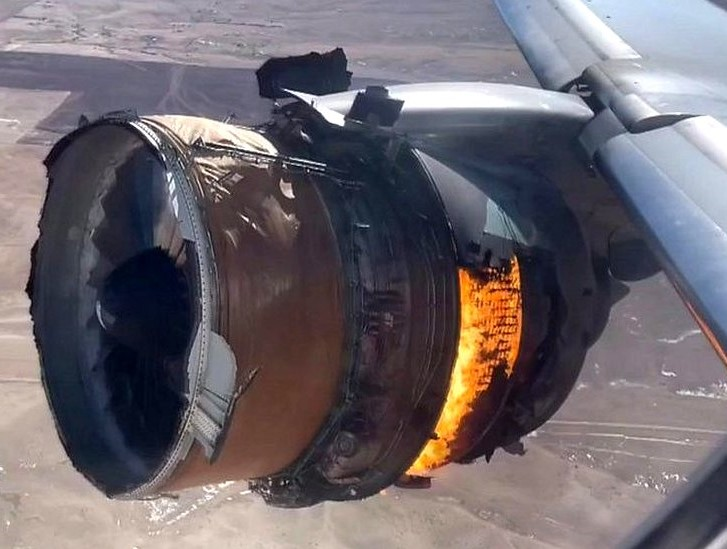
\includegraphics[scale=0.3]{turbine_failure.jpg}
                    \caption{Turbine failure mid-flight \cite{bbc-news-2021}}
                \end{figure}
            \end{column}
        \end{columns}
    \end{frame}

    \begin{frame}{Objectives}

        Develop a ML model to accurately estimate the Remaining Useful Life of a fleet of turbofan engines, applied to PHMAP 2021 dataset:
        \begin{columns}
            \begin{column}{0.5\textwidth}
                \begin{itemize}
                    \item \textbf{Efficient Modelling:} need for lower cost models
                    \item \textbf{Model Interpretability:} understand predictions in critical scenarios
                    \item \textbf{Confidence and prediction intervals:} provide measures of uncertainty
                \end{itemize}
            \end{column}
            \begin{column}{0.5\textwidth}
                \begin{figure}
                    \centering
                    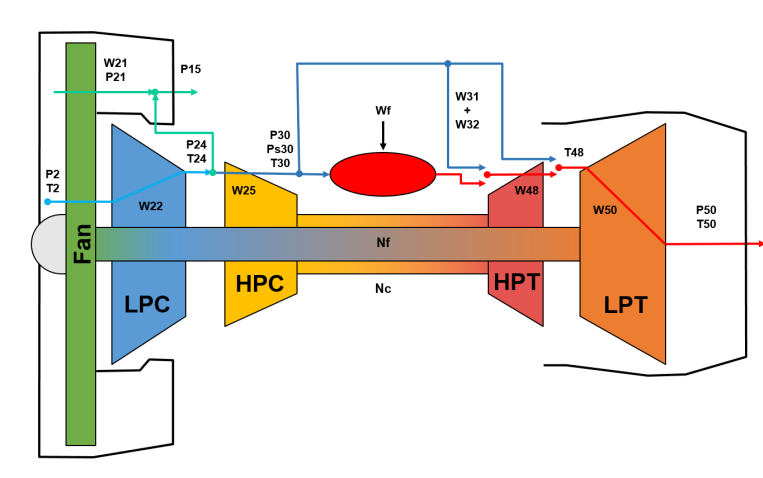
\includegraphics[width=0.9\textwidth]{cmapss_turbofan.png}
                    \caption{Schematics of a turbofan engine}
                \end{figure}
            \end{column}
        \end{columns}
    \end{frame}

    \begin{frame}{Methodology}
        \begin{figure}[!htbp]
            \centering
            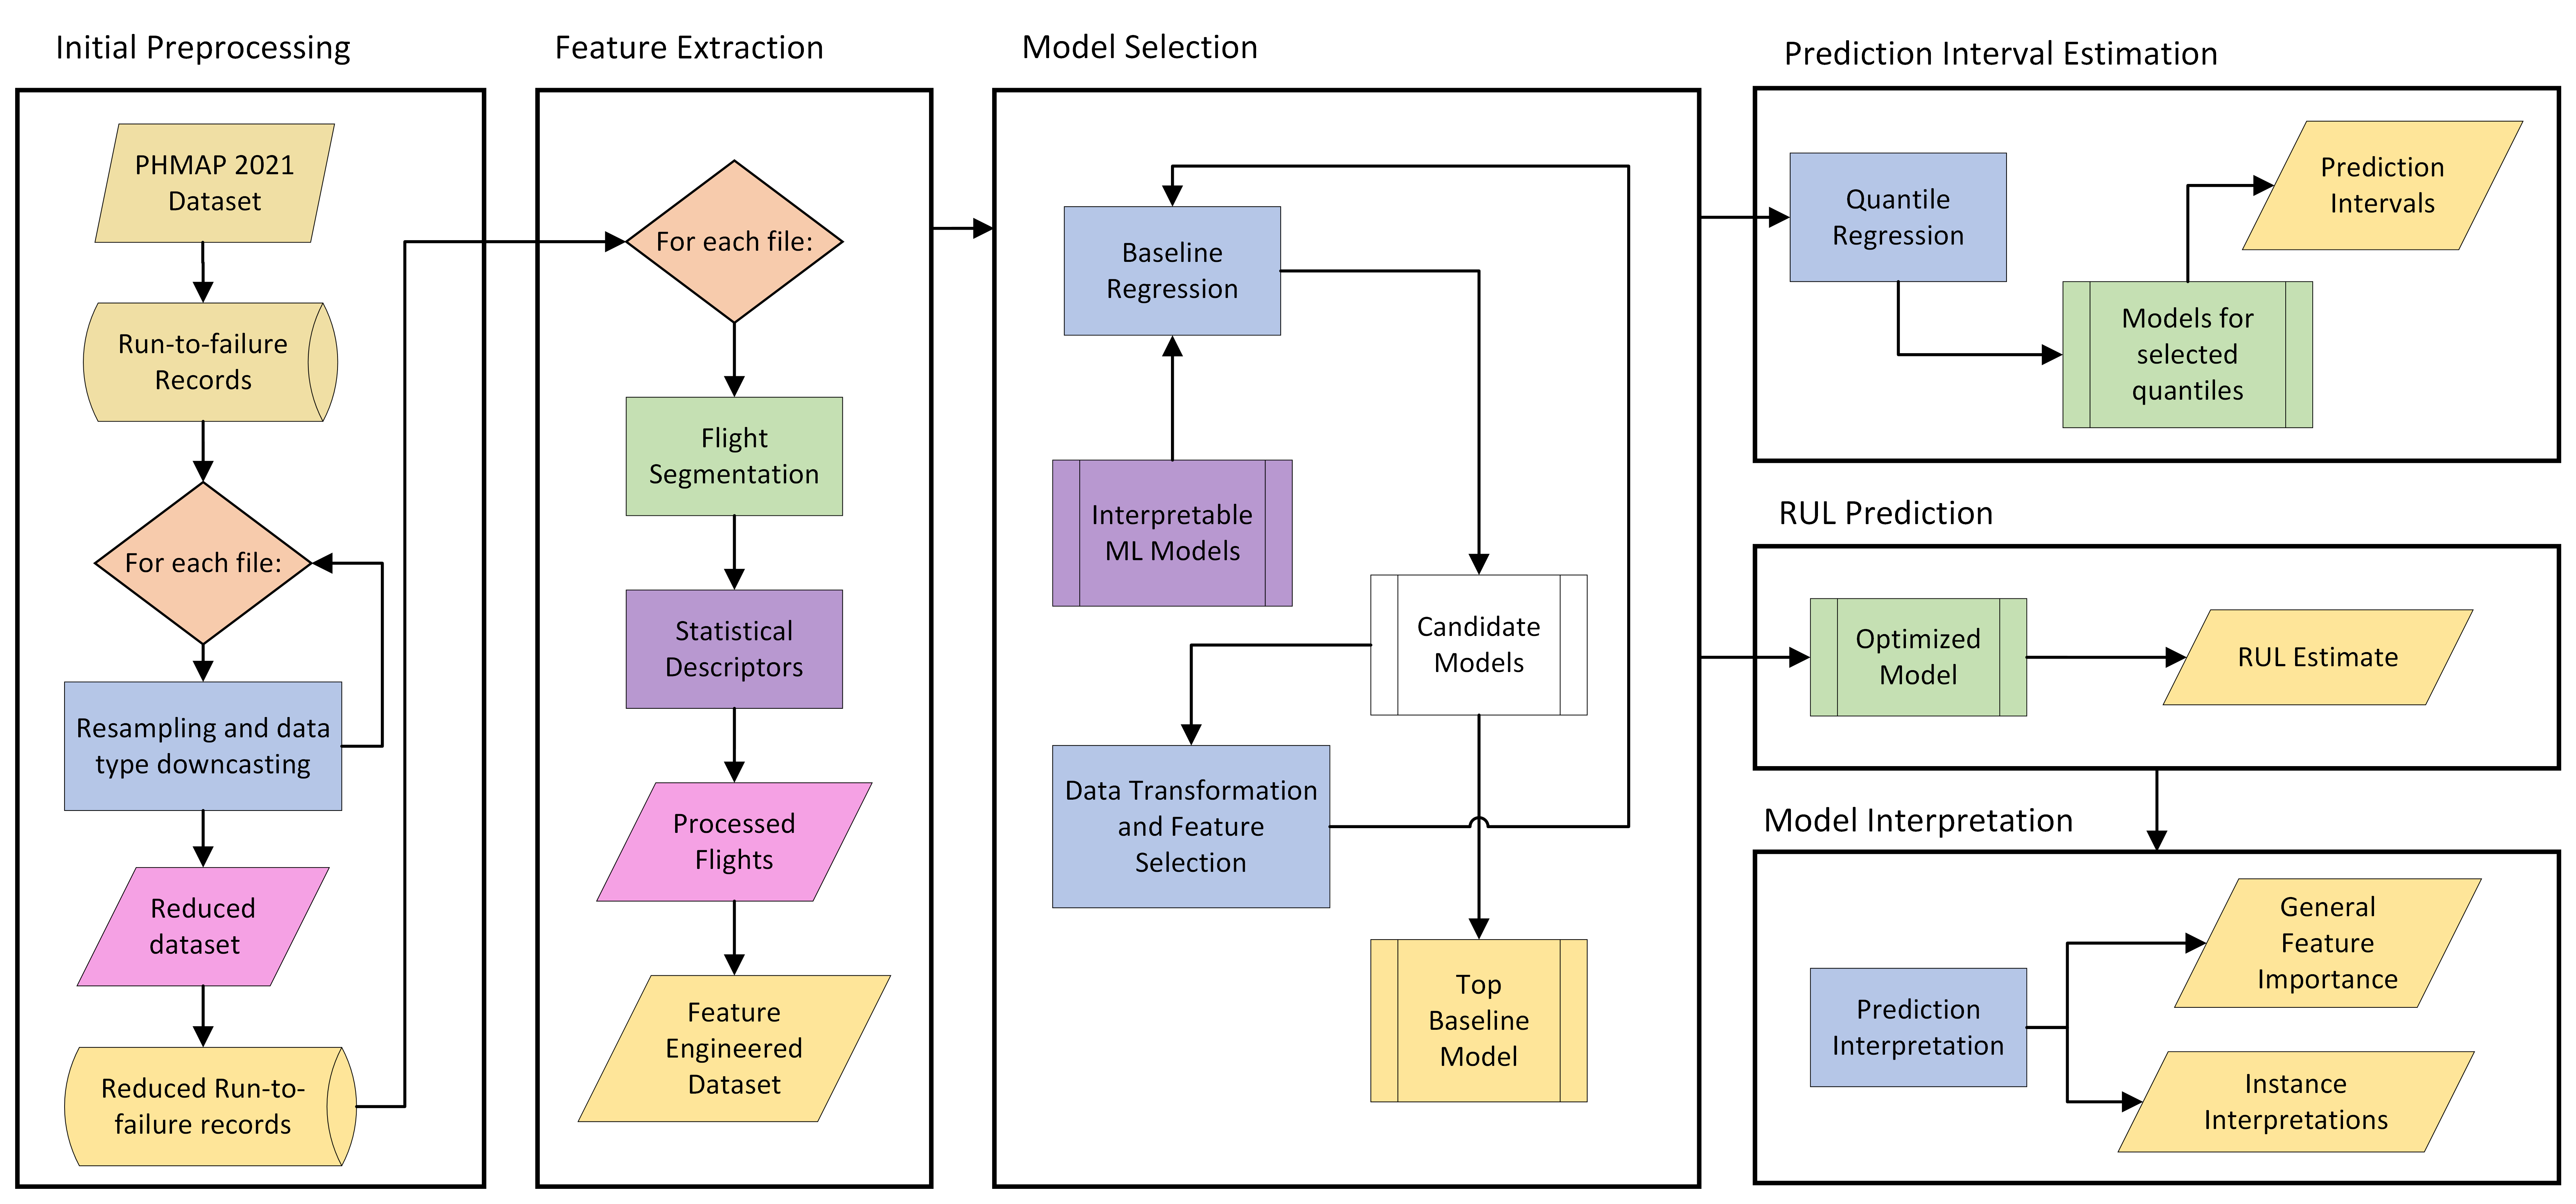
\includegraphics[scale=0.2]{research_diagram.png}
            \caption{Proposed Methodology}
        \end{figure}
    \end{frame}

    \begin{frame}{Results}{RUL / PI estimators}
        \begin{figure}[!htbp]
            \centering
            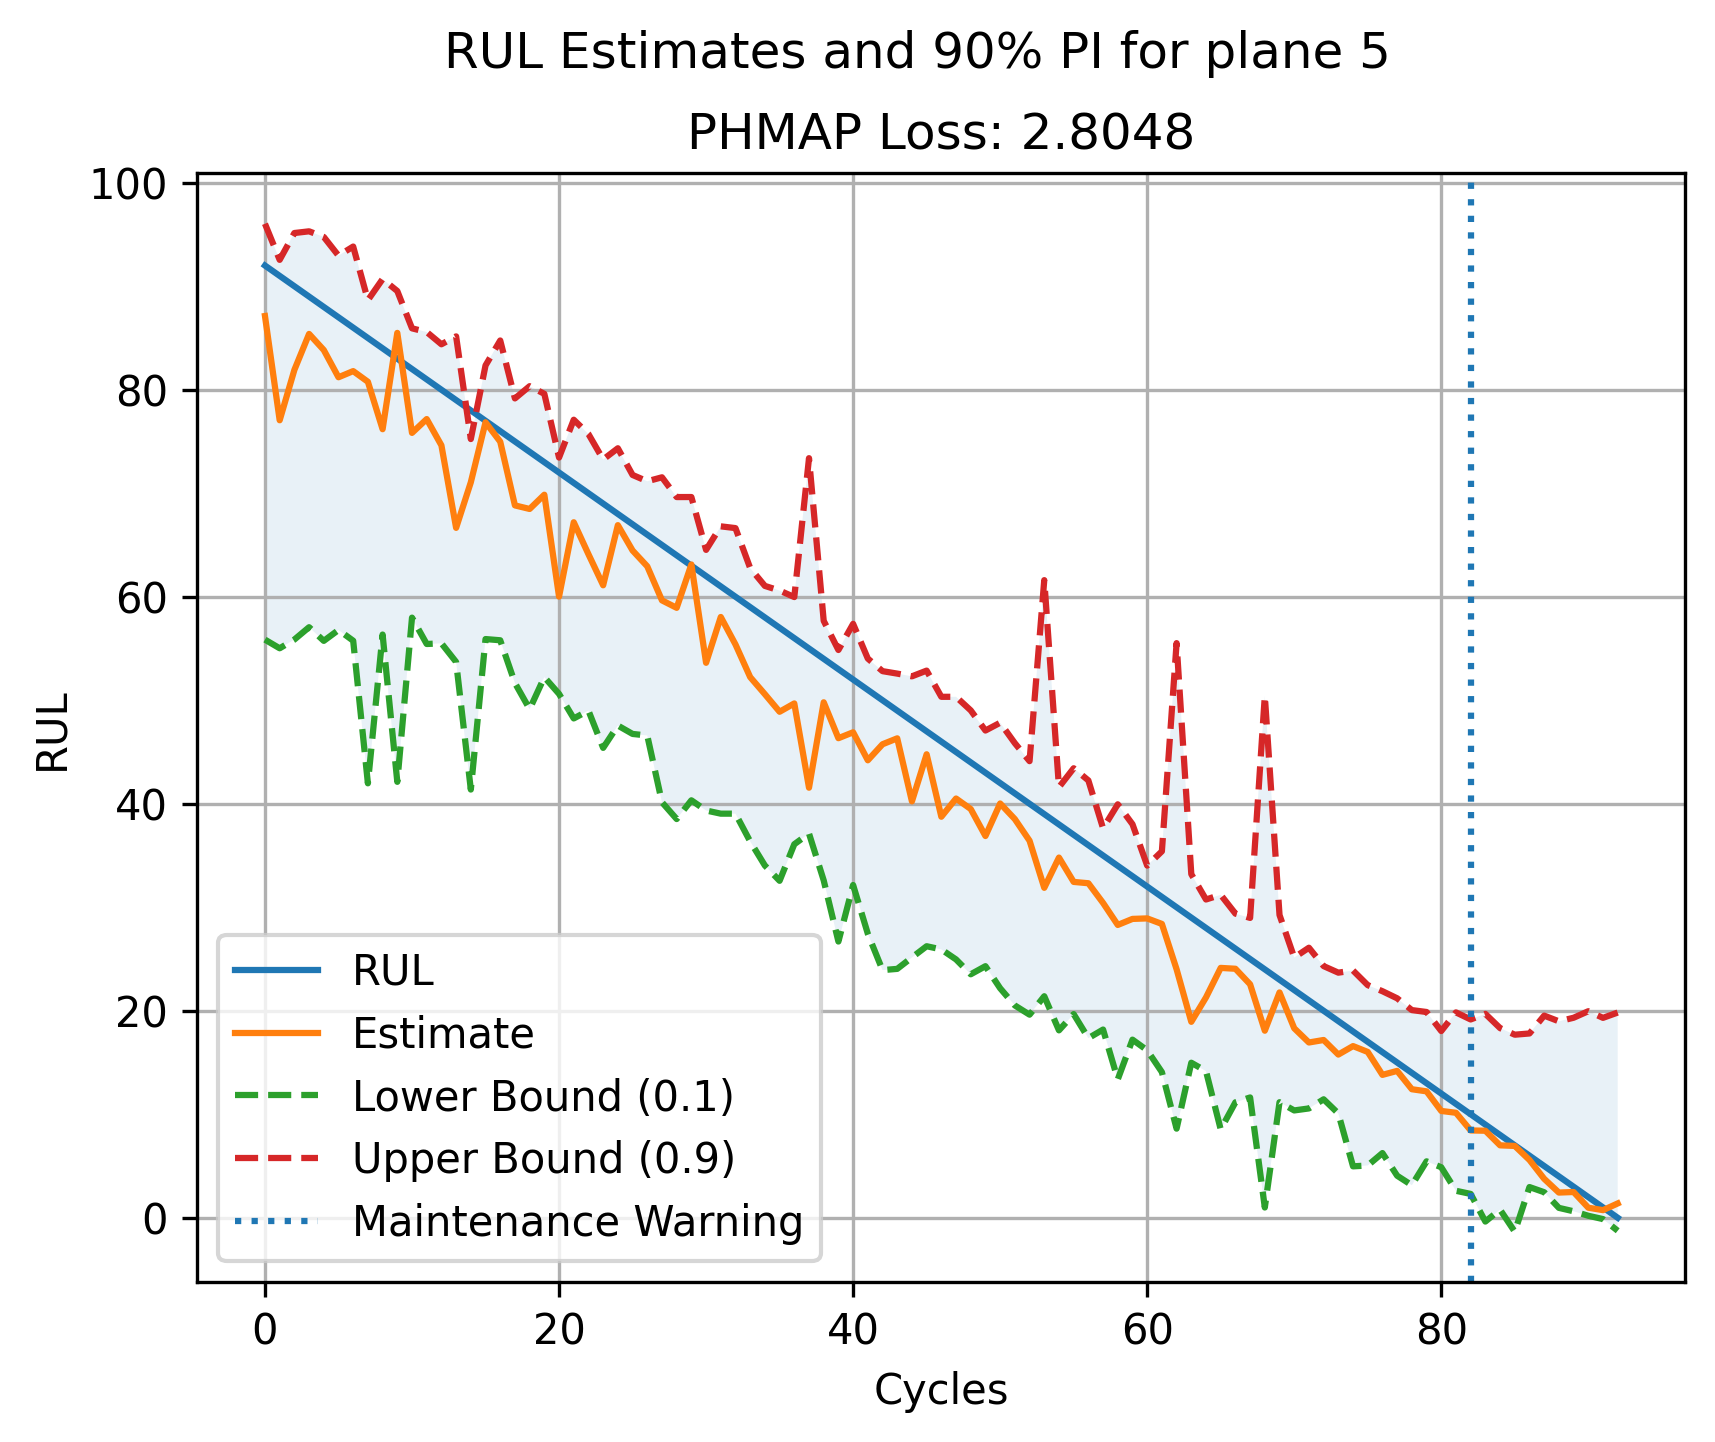
\includegraphics[scale=0.55]{preds_DS03-012_5.png}
            \caption{RUL estimates and PI for the operational life of a plane}
        \end{figure}
    \end{frame}

    \begin{frame}{Model Explainability}
        \begin{figure}[!htbp]
            \centering
            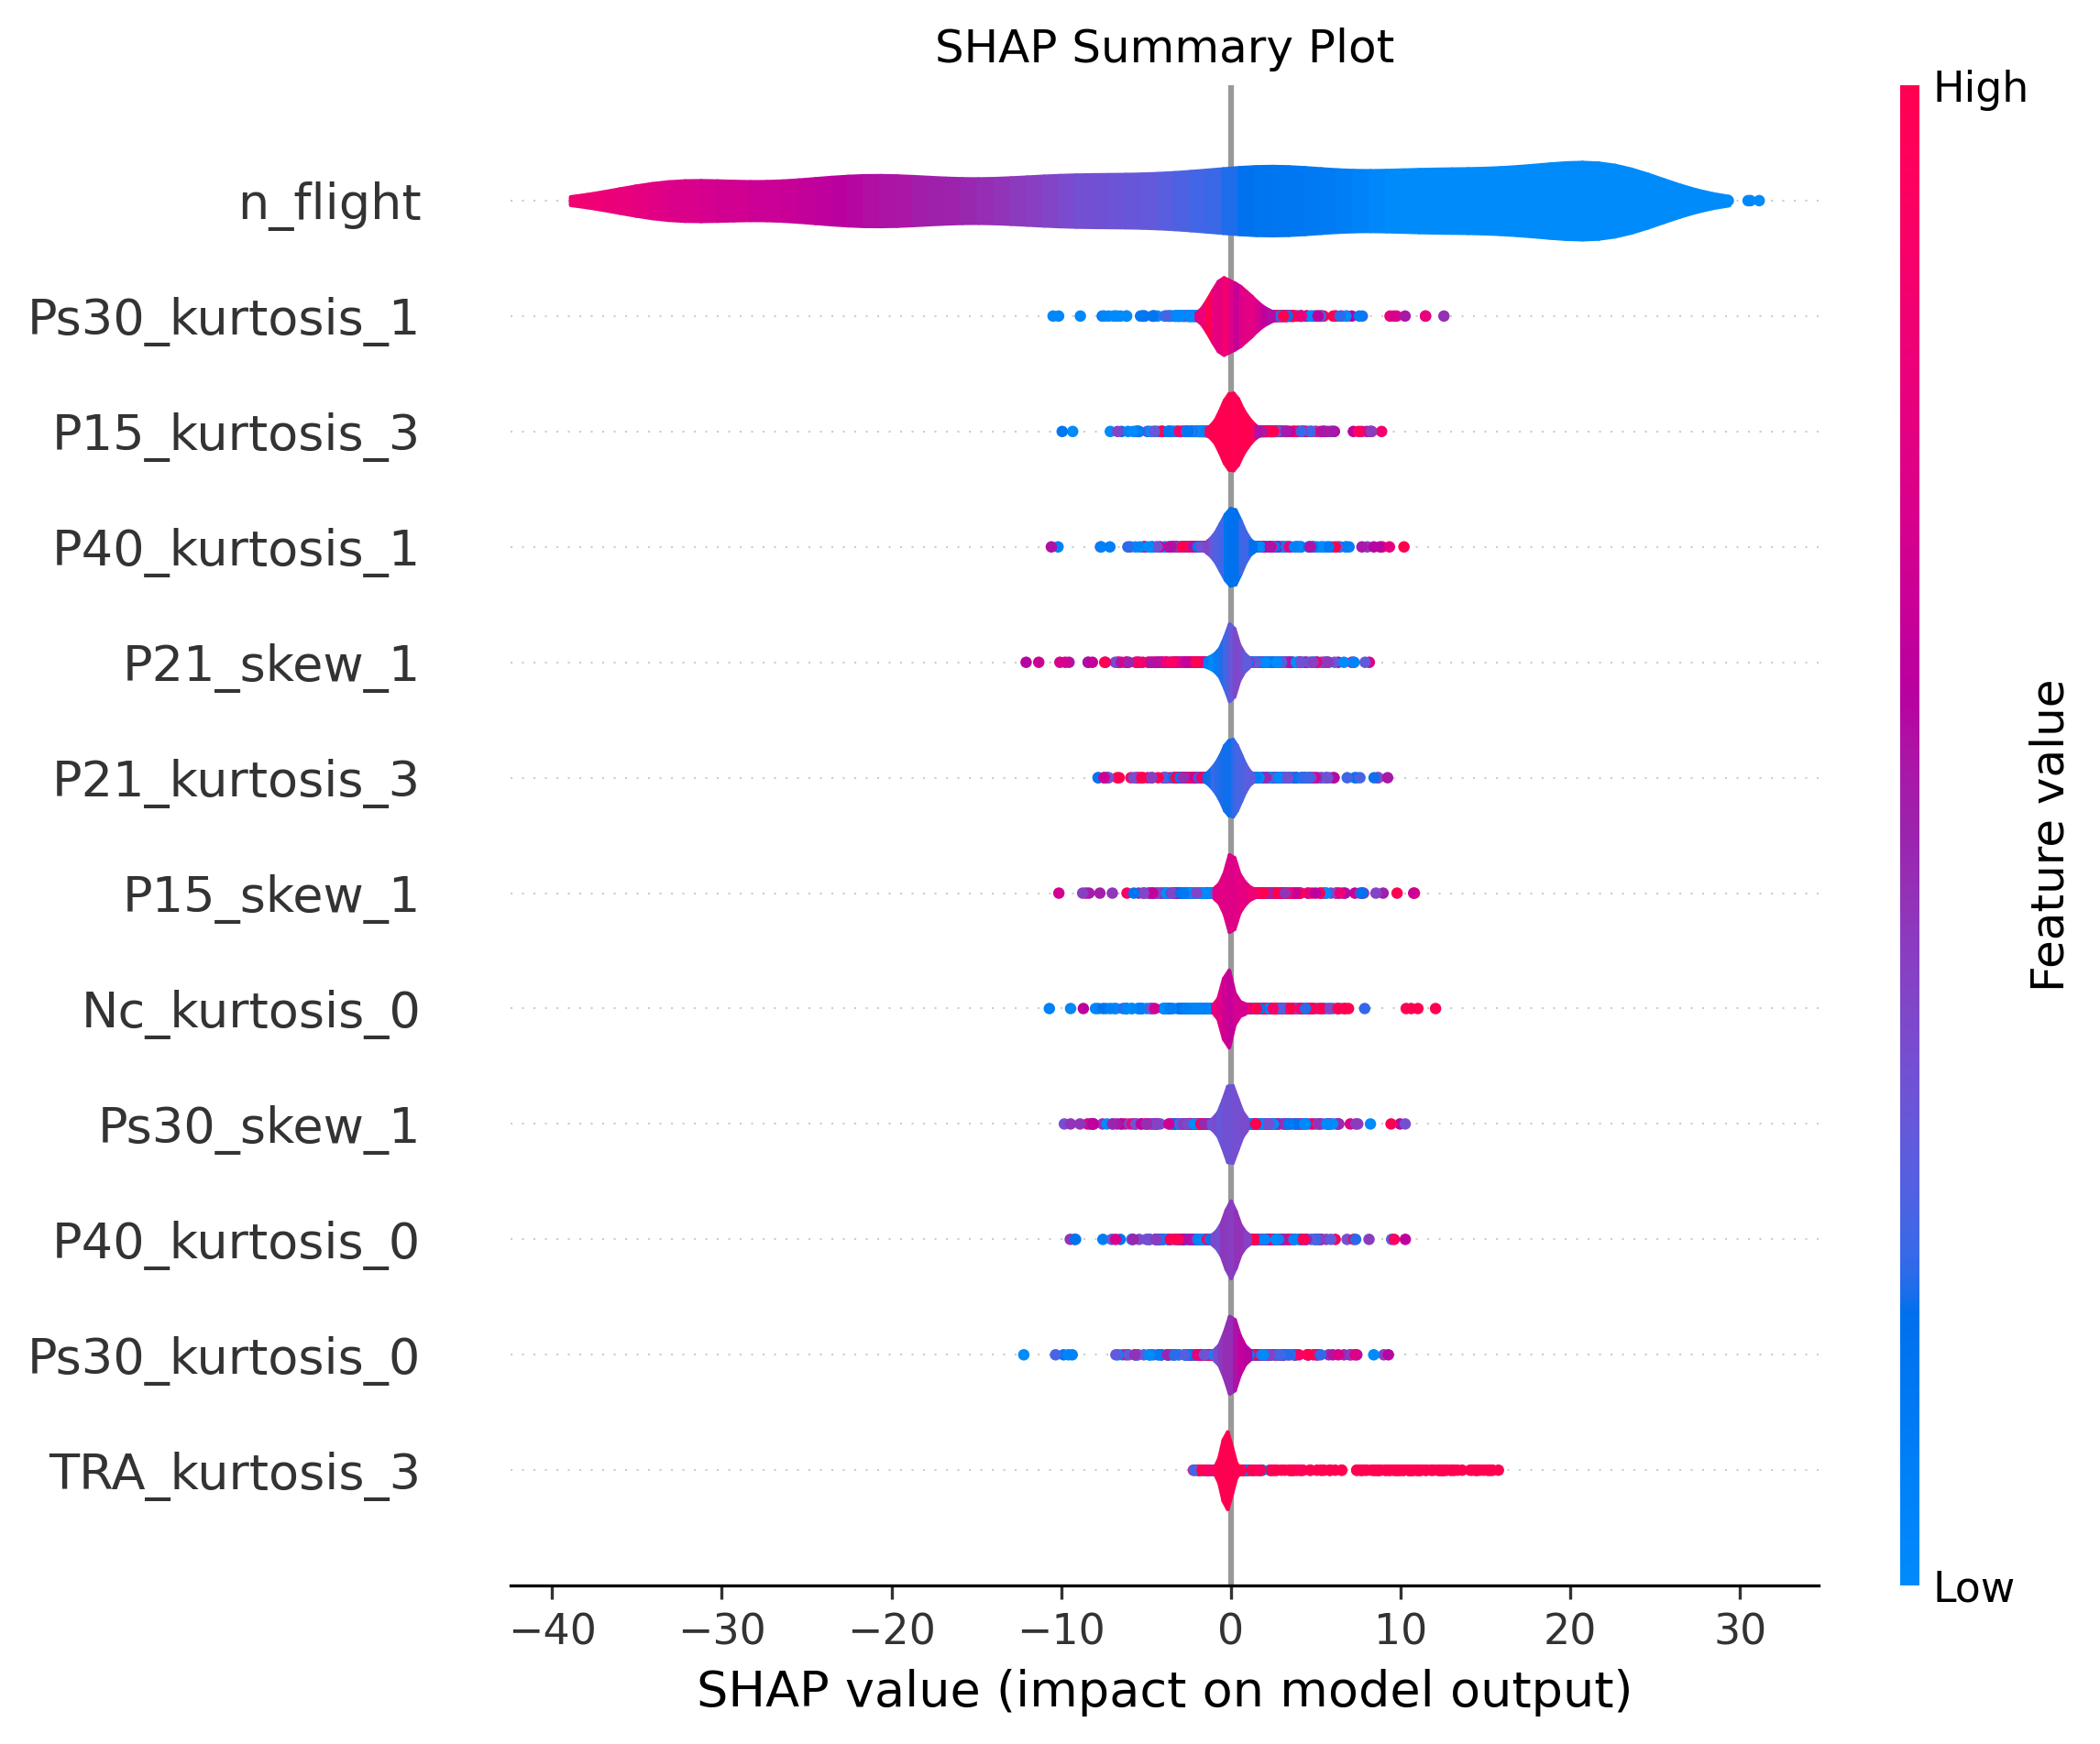
\includegraphics[scale=0.4]{shap_summary.png}
            \caption{SHAP Summary Plot}
        \end{figure}
    \end{frame}

    \section*{References}
    \begin{frame}[allowframebreaks]
        \frametitle{References}
        \printbibliography
    \end{frame}

\end{document}